% LaTeX Template For MATH 490 @ VCU
\documentclass[11pt]{article}

\usepackage{hyperref}
\usepackage{amsmath}
\usepackage{amsthm}
\usepackage{amssymb}
\usepackage{enumerate}
\usepackage{enumitem}
\usepackage{titlesec}
\usepackage{multicol}
\usepackage{multirow}
\usepackage{mathtools}
\usepackage{mdframed}
\usepackage{tocloft}
\usepackage{tcolorbox}
\usepackage{extarrows}

\setlist{nosep}
\setlist[enumerate]{label=\alph*.}

\renewcommand{\arraystretch}{0.75}

\definecolor{defcolor}{RGB}{255,236,236}    % light red
\definecolor{ngtcolor}{RGB}{255,242,242}    % lighter red
\definecolor{lnkcolor}{RGB}{0,0,180}        % blue
\definecolor{thmcolor}{RGB}{236,236,255}    % light blue
\definecolor{lemcolor}{RGB}{239,239,255}    % lighter blue
\definecolor{procolor}{RGB}{242,242,255}    % lighter lighter blue
\definecolor{crlcolor}{RGB}{245,245,255}    % lighter lighter lighter blue
\definecolor{xmpcolor}{RGB}{255,240,225}    % light orange
\definecolor{rmkcolor}{RGB}{233,255,235}    % light green
\definecolor{axicolor}{RGB}{255,255,233}    % light yellow
\definecolor{notcolor}{RGB}{255,255,244}    % lighter yellow
\definecolor{whacolor}{RGB}{250,250,250}    % lighter gray
\definecolor{reccolor}{RGB}{255,244,255}    % lighter purple

\hypersetup{
    colorlinks,
    citecolor=lnkcolor,
    filecolor=lnkcolor,
    linkcolor=lnkcolor,
    urlcolor=lnkcolor
}

\newtheoremstyle{break}
    {\topsep/1.5} % space above
    {\topsep/2.2} % space below
    {}          % body font
    {}          % indent amount
    {\rmfamily} % theorem head font
    {.}          % punctuation after theorem head
    {0.5em}  % space after theorem head
    {\textbf{\thmname{#1}\thmnumber{ #2}}\thmnote{\text{ (#3)}}}
                % theorem hed spec. (empty = "normal")

\theoremstyle{break}
\newmdtheoremenv{theorem}{Theorem}
\newmdtheoremenv{corollary}[theorem]{Corollary}
\newmdtheoremenv{lemma}[theorem]{Lemma}
\newmdtheoremenv{axiom}[theorem]{Axiom}
\newmdtheoremenv{notation}[theorem]{Notation}
\newmdtheoremenv{definition}[theorem]{Definition}
\newmdtheoremenv{remark}[theorem]{Remark}
\newmdtheoremenv{example}[theorem]{Example}
\newmdtheoremenv{problem}[theorem]{Problem}
\newmdtheoremenv{question}[theorem]{Question}

\DeclareMathOperator{\arcsec}{arcsec}
\DeclareMathOperator{\arccot}{arccot}
\DeclareMathOperator{\arccsc}{arccsc}
\DeclareMathOperator{\interior}{int}
\DeclareMathOperator{\closure}{cl}
\DeclareMathOperator{\boundary}{bd}

\newcommand{\dd}{\text{d}}
\newcommand{\ddi}{\text{$\,$d}}
\newcommand{\qqed}{{\hfill$\blacksquare$}}
\newcommand{\defeq}{\overset{\text{def}}{=}}
\newcommand{\transpose}{\text{T}}

\linespread{1.9}
\setlength{\textwidth}{6.9in}
\setlength{\textheight}{9.2in}
\setlength{\oddsidemargin}{-0.2in}
\setlength{\evensidemargin}{-0.2in}
\setlength{\topmargin}{-0.2in}
\setlength{\headheight}{0in}
\setlength{\headsep}{0in}
\setlength{\footskip}{0.5in}
\setlength{\multicolsep}{6.2pt}
\setlength{\belowdisplayskip}{0pt}
%\setlength{\belowdisplayshortskip}{0pt}
\setlength{\abovedisplayskip}{0pt}
%\setlength{\abovedisplayshortskip}{0pt}

\setcounter{section}{0}
\numberwithin{equation}{theorem}

\makeatletter
\newcommand{\vast}{\bBigg@{4}}
\newcommand{\Vast}{\bBigg@{5}}
\makeatother
\title{Homework 1 of Computational Mathematics}
\author{Chang, Yung-Hsuan\\111652004\\Department of Applied Mathematics}

\begin{document}
\maketitle
\thispagestyle{empty}
\newpage
\pagenumbering{arabic}

\begin{problem}\label{problem 1}
    Use the intermediate value theorem and Rolle's theorem to show the graph of \vspace{-0.6em}
    \begin{equation*}
        f(x)=x^3+2x+k \vspace{-0.6em}
    \end{equation*}
    crosses the $x$-axis exactly once, regardless of the value of the constant $k$.
\end{problem}
\textbf{Proof}. Let $k\in\mathbb R$. We first show that $f(x)=0$ has a root. Suppose $k=0$. Then, we can factorize $f(x)=x(x^2+2)$. Thus, it is clear that $f(x)=0$ has only one root $x=0$. Suppose $k>0$. Choose $x_1=0$ and $x_2=-k$. Then, $f(x_1)=k>0$ and $f(x_2)=-k^3-k<0$. By the intermediate value theorem, there exists a root between $x_1$ and $x_2$. Suppose $k<0$. Choose $x_3=0$ and $x_4=-k$. Then, $f(x_3)=k<0$ and $f(x_4)=-k^3-k>0$. By the intermediate value theorem, there exists a root between $x_3$ and $x_4$. We now show that there is only one root. Observe that $\dfrac{\dd f}{\dd x}(x)=3x^2+2>0$ for all $x\in\mathbb R$ regardless of the value of $k$. For the sake of contradiction, we suppose there are two distinct roots $\alpha$ and $\beta$ such that $f(\alpha)=f(\beta)=0$. By Rolle's theorem, there exists an $x_0$ between $\alpha$ and $\beta$ such that $\dfrac{\dd f}{\dd x}(x_0)=0$, a contradiction. Hence, there is only one root. \qed

\newpage
\begin{problem}\label{problem 2}
    Find $\displaystyle\max_{a\leq x\leq b}|f(x)|$ for the following functions and intervals.
    \begin{enumerate}
        \item $f(x)=\dfrac{2-e^x+2x}{3}$, $[0, 1]$
        \item $f(x)=\dfrac{4x-3}{x^2-2x}$, $[0.5, 1]$
        \item $f(x)=2x\cos(2x)-(x-2)^2$, $[2, 4]$
        \item $f(x)=1+e^{-\cos(x-1)}$, $[1, 2]$
    \end{enumerate}
\end{problem}
\textbf{Solution}. Note that we can first looking for extrema for original functions and then find $\displaystyle\max_{a\leq x\leq b}|f(x)|$.
\begin{enumerate}
    \item We first look for critical points. Set $\dfrac{\dd f}{\dd x}(x)(x)=0$ on $[0, 1]$. Then, \vspace{-0.6em}
    \begin{align*}
        \dfrac{-e^x+2}{3}&=0\\
        \iff \quad\quad\quad\quad x&=\ln2.
    \end{align*}
    Then, we have $f(\ln 2)=\dfrac{2\ln 2}{3}\approx0.462$, $f(0)=\dfrac{1}{3}\approx0.333$, and $f(1)=\dfrac{4-e}{3}\approx0.427$. Hence, $\displaystyle\max_{0\leq x\leq 1}|f(x)|=\dfrac{2\ln 2}{3}$.
    \item Observe that the derivative $\dfrac{\dd f}{\dd x}(x)=\dfrac{-4x^2+6x-6}{(x^2-2x)^2}$ has no roots on $\mathbb R$. Hence, the function is monotonic and thus achieves extrema at end points. We have $|f(0.5)|=\dfrac{4}{3}$ and $|f(1)|=1$. Hence, $\displaystyle\max_{0.5\leq x\leq 1}|f(x)|=\dfrac{4}{3}$.
    \item We first look for critical points. Set $\dfrac{\dd f}{\dd x}(x)=0$ on $[2, 4]$. Then, \vspace{-0.6em}
    \begin{equation}\label{eq: problem 2 c 1}
        2\cos(2x)-4x\sin(2x)-2(x-2)=0 \vspace{-0.6em}
    \end{equation}
    Let $x^\ast\in[2, 4]$ satisfies (\ref{eq: problem 2 c 1}). Then, $f(x^\ast)\approx4.981$. We have $f(x^\ast)\approx4.981$, $f(2)\approx-2.615$, and $f(4)\approx-5.164$. Hence, $\displaystyle\max_{2\leq x\leq 4}|f(x)|=4-8\cos(8)$.
    \item We first look for critical points. Set $\dfrac{\dd f}{\dd x}(x)=0$ on $[1, 2]$. Then, \vspace{-0.6em}
    \begin{align*}
        e^{-\cos(x-1)}\cdot\sin(x-1)&=0\\
        \iff\quad\quad\quad\quad\quad\quad\sin(x-1)&=0\\
        \implies\quad\quad\quad\quad\quad\quad\quad\quad\quad\ \  x&=1.\\[-3.4em]
    \end{align*}
    Then, we have $f(1)=1+e^{-1}\approx1.368$, $f(2)=1+e^{-\cos1}\approx1.583$. Hence, $\displaystyle\max_{1\leq x\leq 2}|f(x)|=1+e^{-\cos1}$. \qed
\end{enumerate}

\newpage
\begin{problem}\label{problem 3}
    Find the second Taylor polynomial $P_2(x)$ for the function $f(x)=e^x\cos(x)$ about $x_0=0$.
    \begin{enumerate}
        \item Use $P_2(0.5)$ to approximate $f(0.5)$. Find an upper bound for error $|f(0.5)-P_2(0.5)|$ using the error formula, and compare it to the actual error.
        \item Find a bound for the error $|f(0.5)-P_2(0.5)|$ in using $P_2(x)$ to approximate $f(x)$ on the interval $[0, 1]$.
        \item Approximate $\displaystyle\int_{0}^{1}f(x)\ddi x$ using $\displaystyle\int_{0}^{1}P_2(x)\ddi x$.
        \item Find an upper bound for the error in (c) using $\displaystyle\int_{0}^{1}|R_2(x)|\ddi x$.
    \end{enumerate}
\end{problem}
\textbf{Solution}. By Taylor's theorem, we have \vspace{-0.6em}
\begin{align*}
    e^x\cos x&=f(0)+\dfrac{1}{1!}\cdot\dfrac{\dd f}{\dd x}(0)\cdot x+\dfrac{1}{2!}\cdot\dfrac{\dd^2 f}{\dd x^2}(0)\cdot x^2+\dfrac{1}{3!}\cdot\dfrac{\dd^3 f}{\dd x^3}(\xi(x))\cdot x^3\\
    &=1+x+\dfrac{1}{6}\cdot\left(-2e^{\xi(x)}\left(\sin \xi(x)+\cos \xi(x)\right) \right) \cdot x^3\\
    &=1+x-\dfrac{\sqrt{2}}{3}\cdot e^{\xi(x)}\sin\left(\xi(x)+\dfrac{\pi}{4}\right) \cdot x^3\\[-3.4em]
\end{align*}
Hence, the second Taylor polynomial about $0$ is \vspace{-0.6em}
\begin{equation*}
    P_2(x)=1+x. \vspace{-0.6em}
\end{equation*}
\begin{enumerate}
    \item The value of the second Taylor polynomial $P_2(0.5)=1.5$, and the true value $f(0.5)\approx1.446889$. We can estimate the upper bound of $|f(0.5)-P_2(0.5)|$ by \vspace{-0.6em}
    \begin{align*}
        |f(0.5)-P_2(0.5)|&=\left\lvert \dfrac{\sqrt{2}}{3}\cdot e^{\xi(0.5)}\sin\left(\xi(0.5)+\dfrac{\pi}{4}\right) \cdot ({0.5})^3\right\rvert\\
        &\leq\left\lvert \dfrac{\sqrt{2}}{3}\cdot e^{0.5}\sin\left(0.5+\dfrac{\pi}{4}\right) \cdot ({0.5})^3\right\rvert\\
        &\leq 0.093222005.\\[-3.4em]
    \end{align*}
    The actual error is $\left\lvert e^{0.5}\cos(0.5)-1.5\right\rvert\approx0.0531111$ and is smaller than the upper bound.
    \item For $t\in[0, 1]$, the maximum of $e^t$ is $e^1=e$, the maximum of $\sin\left(t+\dfrac{\pi}{4}\right)$ is $\sin\left(\dfrac{\pi}{4}+\dfrac{\pi}{4}\right)=1$, and the maximum of $t^3$ is $1^3=1$. Hence, the maximum of $\dfrac{\sqrt{2}}{3}\cdot e^{\xi(x)}\sin\left(\xi(x)+\dfrac{\pi}{4}\right) \cdot x^3$ on $x\in[0, 1]$ is $\dfrac{\sqrt{2}}{3}\cdot e\cdot1\cdot1^3\approx1.281410342720$.
    \item \begin{align*}
        \int_{0}^{1}P_2(x)\ddi x&=\int_{0}^{1}1+x\ddi x\\
        &=\left[x+\dfrac{x^2}{2}\right]_0^1\\
        &=\dfrac{3}{2}.
    \end{align*}
    \item The error is approximately \vspace{-0.6em}
    \begin{align*}
        \left|\int_{0}^{1}f(x)\ddi x-\int_{0}^{1}P_2(x)\ddi x\right|&\leq\int_{0}^{1}|R_2(x)|\ddi x\\
        &=\dfrac{\sqrt{2}}{3}\int_{0}^{1}\left|e^x\sin\left(x+\dfrac{\pi}{4}\right) \cdot x^3\right|\ddi x\\
        &\overset{\mathcal{M}}{\approx}0.2625,\\[-3.4em]
    \end{align*}
    where $\overset{\mathcal{M}}{\approx}$ suggests that the value is computed and approximated by MATLAB. See Figure 3.d.1.
    \begin{center}
        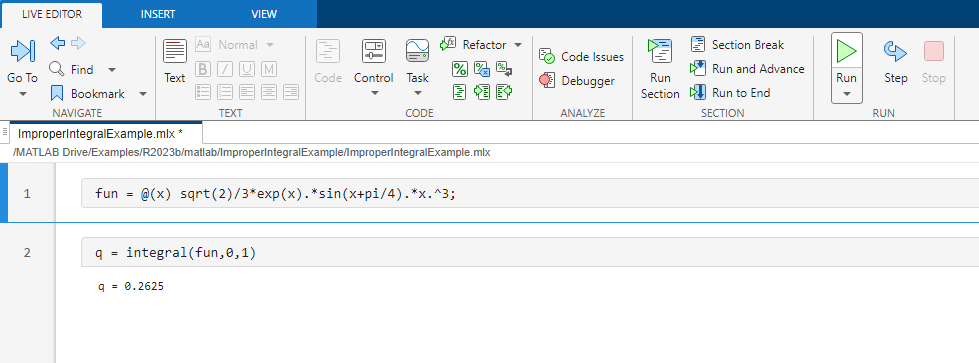
\includegraphics[width=0.8\textwidth]{P3d1.png}\\
        Figure 3.d.1.
    \end{center}
    Hence, an upper bound is $0.27$. \qed
\end{enumerate}

\newpage
\begin{problem}\label{problem 4}
    Let $f(x)=\dfrac{1}{1-x}$ and $x_0=0$. Find the $n$-th Taylor polynomial $P_n(x)$ for $f(x)$ about $x_0$. Find a value of $n$ necessary for $P_n(x)$ to approximate $f(x)$ to within $10^{-6}$ on $[0, 0.5]$.
\end{problem}
\textbf{Solution}. Notice that $f(x)=\dfrac{1}{1-x}$ is the infinite sum of $\{x^k\}_{k=0}^\infty$. Hence, the $n$-th Taylor polynomial is $\displaystyle P_n(x)=1+x+\cdots+x^n$. We would like to find an $n\in\mathbb{N}$ such that $|P_n(x)-f(x)|<10^{-6}$ for all $x\in[0, 0.5]$. Observe that $f(x)>P_n(x)$ for all $x\in[0, 5]$, and $\dfrac{\dd}{\dd x}\left(f(x)-P_n(x)\right)\geq 0$ for all $x\in[0, 0.5]$. Hence, \vspace{-0.6em}
\begin{align*}
    \sup_{x\in[0, 0.5]}|P_n(x)-f(x)|&=f(0.5)-P_n(0.5)\\
    &=2-\sum_{i=0}^{n}(0.5)^i\\
    &=2-\dfrac{1-0.5^{n+1}}{1-0.5}\\
    &=0.5^n.\\[-3.4em]
\end{align*}
Set $0.5^n<10^{-6}$. Then, we obtain that the integer $n$ must be greater than $19$. Hence, we choose $n=20$ as the desired exponent. \qed

\newpage
\begin{problem}\label{problem 5}
    Find the largest interval in which $p^\ast$ must lie to approximate $p$ with relative error at most $10^{-4}$ for each value of $p$.
    \begin{enumerate}
        \item $\pi$
        \item $e$
        \item $\sqrt{2}$
        \item $\sqrt[3]{7}$
    \end{enumerate}
\end{problem}
\textbf{Solution}. The relative of $p^\ast$ for $p$ is $\left|\dfrac{p^{\ast}-p}{p}\right|$. Set \vspace{-0.6em}
\begin{equation*}
    \left|\dfrac{p^{\ast}-p}{p}\right|\leq 10^{-4}. \vspace{-0.6em}
\end{equation*}
Then, \vspace{-0.6em}
\begin{align*}
    \left|p^{\ast}-p\right|\leq p\cdot 10^{-4}\\
    p-p\cdot 10^{-4}\leq p^\ast\leq p+p\cdot 10^{-4}\\[-3.4em]
\end{align*}
whenever $p\geq 0$. Hence, by the fact that all $p^\ast$'s are greater than $0$, the desired interval for each is
\begin{enumerate}
    \item $\left[\pi-\pi\cdot10^{-4}, \pi+\pi\cdot10^{-4}\right]$;
    \item $\left[e-e\cdot10^{-4}, e+e\cdot10^{-4}\right]$;
    \item $\left[\sqrt{2}-\sqrt{2}\cdot10^{-4}, \sqrt{2}+\sqrt{2}\cdot10^{-4}\right]$; and
    \item $\left[\sqrt[3]{7}-\sqrt[3]{7}\cdot10^{-4}, \sqrt[3]{7}+\sqrt[3]{7}\cdot10^{-4}\right]$. \qed
\end{enumerate}

\newpage
\begin{problem}\label{problem 6}
    Let \vspace{-0.6em}
    \begin{equation*}
        f(x)=\dfrac{e^{x}-e^{-x}}{x}. \vspace{-0.6em}
    \end{equation*}
    \begin{enumerate}
        \item Find $\displaystyle\lim_{x\to 0}\dfrac{e^{x}-e^{-x}}{x}$.
        \item Use three-digit rounding arithmatic to evaluate $f(0.1)$.
        \item Replace each exponential function with its third Maclaurin polynomial, and repeat part (b).
        \item The actual value is $f(0.1)=2.003335000$. Find the relative error for the values obtained in part (b) and (c).
    \end{enumerate}
\end{problem}
\textbf{Solution}.
\begin{enumerate}
    \item Using l'Hôpital's rule, \vspace{-0.6em}
    \begin{align*}
        \lim_{x\to 0}\dfrac{e^x-e^{-x}}{x}&\overset{L'}{=}\lim_{x\to 0}\dfrac{e^x+e^x}{1}\\
        &=2.\\[-3.4em]
    \end{align*}
    \item Plug in the value $x=0.1$, by calculator, $f(0.1)\overset{\textbf{R}_3}{\approx}\dfrac{1.11-0.905}{0.10}=2.05$, where $\overset{\textbf{R}_3}{\approx}$ denotes three-digit rounding arithmatic.
    \item Plug in the value $x=0.1$ with substitution $e^x=1+x+\dfrac{x^2}{2}+\dfrac{x^3}{6}$, we have \vspace{-0.6em}
    \begin{align*}
        f(0.1)&\overset{\textbf{M}_{3}}{\approx}\dfrac{1+0.1+\dfrac{0.01}{2}+\dfrac{0.001}{6}-1+0.1-\dfrac{0.01}{2}+\dfrac{0.001}{6}}{0.1}\\
        &=\dfrac{0.1+0.1+0.000167+0.000167}{0.1}\\
        &\overset{\textbf{R}_3}{\approx}2.00,\\[-3.4em]
    \end{align*}
    where $\overset{\textbf{M}_{3}}{\approx}$ denotes approximation with its third Maclaurin polynomial.
    \item The relative error in part (b) is \vspace{-0.6em}
    \begin{equation*}
        \left|\dfrac{2.003335000-2.05}{2.003335000}\right|\approx0.02329365783; \vspace{-0.6em}
    \end{equation*}
    the relative error in part (c) is \vspace{-0.6em}
    \begin{equation*}
        \left|\dfrac{2.003335000-2.00}{2.003335000}\right|\approx0.001664724073. \vspace{-0.6em}
    \end{equation*}
    \qed
\end{enumerate}

\newpage
\begin{problem}\label{problem 7}
    Use the 64-bit long real format to find the decimal equivalent of the following floating-point machine numbers.
    \begin{enumerate}
        \item $0\quad 10000001010\quad 1001001100000000000000000000000000000000000000000000$
        \item $1\quad 10000001010\quad 1001001100000000000000000000000000000000000000000000$
        \item $0\quad 01111111111\quad 0101001100000000000000000000000000000000000000000000$
        \item $0\quad 01111111111\quad 0101001100000000000000000000000000000000000000000001$
    \end{enumerate}
\end{problem}
\textbf{Solution}.
\begin{enumerate}
    \item Let $r_a$ be the desired floating-point number. Then, \vspace{-0.6em}
    \begin{align*}
        r_a&=(-1)^0\:2^{c-1023}\:(1+m)\\
        &=2^{11}\cdot1.57421875\\
        &=3224,\\[-3.4em]
    \end{align*}
    where $c=1024+8+2=1034$ and $m=\dfrac{1}{2^{1}}+\dfrac{1}{2^{4}}+\dfrac{1}{2^{7}}+\dfrac{1}{2^{8}}=\dfrac{147}{256}=0.57421875$.
    \item Let $r_b$ be the desired floating-point number. Observe that $r_b=-r_a$. Thus, $r_b=-3224$.
    \item Let $r_c$ be the desired floating-point number. Then, \vspace{-0.6em}
    \begin{align*}
        r_c&=(-1)^0\:2^{c-1023}\:(1+m)\\
        &=2^{0}\cdot1.32421875\\
        &=1.32421875,\\[-3.4em]
    \end{align*}
    where $c=512+256+\cdots+2+1=1023$ and $m=\dfrac{1}{2^{2}}+\dfrac{1}{2^{4}}+\dfrac{1}{2^{7}}+\dfrac{1}{2^{8}}=\dfrac{83}{256}=0.32421875$.
    \item Let $r_d$ be the desired floating-point number. Then, \vspace{-0.6em}
    \begin{align*}
        r_d&=(-1)^0\:2^{c-1023}\:(1+m)\\
        &=2^{0}\cdot1.3242187500000002220446049250313080847263336181640625\\
        &=1.3242187500000002220446049250313080847263336181640625,\\[-3.4em]
    \end{align*}
    where $c=512+256+\cdots+2+1=1023$ and $m=\dfrac{1}{2^{2}}+\dfrac{1}{2^{4}}+\dfrac{1}{2^{7}}+\dfrac{1}{2^{8}}+\dfrac{1}{2^{52}}=\dfrac{2^{50}+2^{48}+2^{45}+2^{44}+1}{2^{52}}=0.3242187500000002220446049250313080847263336181640625$. \qed
\end{enumerate}

\newpage
\begin{problem}\label{problem 8}
    The two-by-two system \vspace{-0.6em}
    \begin{equation*}
        \left\{
            \begin{array}{c}
                ax+by=e;\\
                cx+dy=f,
            \end{array}
        \right. \vspace{-0.6em}
    \end{equation*}
    where $a, b, c, d, e, f$ are given, can be solved for $x$ and $y$ as follows:
    \begin{enumerate}[label=\arabic*.]
        \item Set $m=\dfrac{c}{a}$, provided $a\ne 0$;
        \item $d_1=d-mb$;
        \item $f_1=f-me$;
        \item $y=\dfrac{f_1}{d_1}$; and then
        \item $x=\dfrac{e-by}{a}$.
    \end{enumerate}
    Solve the following linear systems using four-digit rounding arithmetic.
    \begin{enumerate}
        \item $\displaystyle\left\{
            \begin{array}{c}
                1.130x-6.990y=14.20\\
                1.013x-6.099y=14.22
            \end{array}
        \right.$
        \item $\displaystyle\left\{
            \begin{array}{r}
                8.110x+12.20y=-0.1370\\
                -18.11x+112.2y=-0.1376
            \end{array}
        \right.$
    \end{enumerate}
\end{problem}
\textbf{Solution}.
\begin{enumerate}
    \item \begin{enumerate}[label=\arabic*.]
        \item Provided that $a\ne 0$, set $m=\dfrac{1.013}{1.130}\overset{\textbf{R}_4}{\approx}0.8965$;
        \item $d_1=-6.099-0.8965\cdot(-6.990)\overset{\textbf{R}_4}{\approx}0.1680$;
        \item $f_1=14.22-0.8965\cdot14.20\overset{\textbf{R}_4}{\approx}1.490$;
        \item $y=\dfrac{1.490}{0.1680}\overset{\textbf{R}_4}{\approx}8.869$; and then
        \item $x=\dfrac{14.20-(-6.990)\cdot8.869}{1.130}\overset{\textbf{R}_4}{\approx}67.42$.
    \end{enumerate}
    \item \begin{enumerate}[label=\arabic*.]
        \item Provided that $a\ne 0$, set $m=\dfrac{-18.11}{8.110}\overset{\textbf{R}_4}{\approx}-2.233$;
        \item $d_1=112.2-(-2.233)\cdot12.20\overset{\textbf{R}_4}{\approx}139.4$;
        \item $f_1=-0.1376-(-2.233)\cdot(-0.1370)\overset{\textbf{R}_4}{\approx}-0.4435$;
        \item $y=\dfrac{-0.4435}{139.4}\overset{\textbf{R}_4}{\approx}=-0.003181$; and then
        \item $x=\dfrac{-0.1370-12.20\cdot(-0.003181)}{8.110}\overset{\textbf{R}_4}{\approx}-0.01211$. \qed
    \end{enumerate}
\end{enumerate}

\newpage
\begin{problem}\label{problem 9}
    Suppose one calculates in two-digit rounding arithmetic. A rectangular parallelepiped has sides of length $3$ cm, $4$ cm, and $5$ cm, measured to the nearest centimeter. What are the best upper and lower bounds for the volume of this parallelepiped? What are the best upper and lower bounds for the surface area?
\end{problem}
\textbf{Solution}. The true values of the three sides are in $[2.5, 3.5)$ cm, $[3.5, 4.5)$ cm, and $[4.5, 5.5)$ cm, respectively. Hence, for the volume, the best upper bound is $3.5\cdot4.5\cdot5.5\overset{\textbf{R}_2}{\approx}88$, and the best lower bound is $2.5\cdot4.5\cdot3.5\overset{\textbf{R}_2}{\approx}39$; for the surface area, the best upper bound is $2\cdot(3.5\cdot4.5+3.5\cdot5.5+4.5\cdot5.5)=120$, and the best lower bound is $2\cdot(2.5\cdot3.5+2.5\cdot4.5+3.5\cdot4.5)=72$. \qed

\newpage
\begin{problem}\label{problem 10}
    Find the rate of convergence of the following.
    \begin{enumerate}
        \item $\displaystyle\lim_{n\to\infty}\sin\left(\dfrac{1}{n^2}\right)$
        \item $\displaystyle\lim_{n\to\infty}\left(\sin\left(\dfrac{1}{n}\right)\right)^2$
        \item $\displaystyle\lim_{h\to 0}\dfrac{\sin h}{h}$
        \item $\displaystyle\lim_{h\to 0}\dfrac{1-e^h}{h}$
    \end{enumerate}
\end{problem}
\textbf{Solution}.
\begin{enumerate}
    \item Notice that $\displaystyle\lim_{n\to\infty}\sin\left(\dfrac{1}{n^2}\right)=0$. Choose $\{\beta_n\}=\left\{\dfrac{1}{n^2}\right\}$, which converges to $0$. Choose $K=1$. Then, \vspace{-0.6em}
    \begin{align*}
        \left\lvert\sin\left(\dfrac{1}{n^2}\right)-0\right\rvert&=\left\lvert\sin\left(\dfrac{1}{n^2}\right)\right\rvert\\
        &<1\cdot\dfrac{1}{n^2}\\[-3.4em]
    \end{align*}
    for all $n\in\mathbb{N}$. Hence, $\left\{\sin\left(\dfrac{1}{n^2}\right)\right\}_{n=1}^\infty$ converges to $0$ with a rate of convergence $\mathcal{O}\left(\dfrac{1}{n^2}\right)$.
    \item Notice that $\displaystyle\lim_{n\to\infty}\left(\sin\left(\dfrac{1}{n}\right)\right)^2=0$. Choose $\{\beta_n\}=\left\{\dfrac{1}{n^2}\right\}$, which converges to $0$. Choose $K=1$. Then, \vspace{-0.6em}
    \begin{align*}
        \left\lvert\left(\sin\left(\dfrac{1}{n}\right)\right)^2-0\right\rvert&=\left(\sin\left(\dfrac{1}{n}\right)\right)^2\\
        &<\left(\dfrac{1}{n}\right)^2\\
        &=1\cdot\dfrac{1}{n^2}\\[-3.4em]
    \end{align*}
    for all $n\in\mathbb{N}$. Hence, $\left\{\left(\sin\left(\dfrac{1}{n}\right)\right)^2\right\}_{n=1}^\infty$ converges to $0$ with a rate of convergence $\mathcal{O}\left(\dfrac{1}{n^2}\right)$.
    \item Notice that $\displaystyle\lim_{h\to 0}\dfrac{\sin h}{h}=1$. Choose $G(h)=h^2$, of which the limit is $0$ as $h\downarrow 0$. Choose $K=1$. We first Taylor expend $\sin h$ about $x_0=0$: \vspace{-0.6em}
    \begin{equation*}
        \sin h\approx h-\dfrac{h^3}{3!}+\dfrac{h^5}{5!}-\cdots. \vspace{-0.6em}
    \end{equation*}
    Then, \vspace{-0.6em}
    \begin{align*}
        \left\lvert \dfrac{\sin h}{h}-1\right\rvert&=\left\lvert -\dfrac{h^2}{3!}+\dfrac{h^4}{5!}-\cdots\right\rvert\\
        &<1\cdot h^2+\mathcal{O}(h^4)\\[-3.4em]
    \end{align*}
    for $h\in(0, 1)$. Note that $h^2+\mathcal{O}(h^4)=\mathcal{O}(h^2)$. Hence, $\displaystyle\lim_{h\to 0}\dfrac{\sin h}{h}=1$ with a rate of convergence $\mathcal{O}(h^2)$.
    \item Notice that $\displaystyle\lim_{h\to 0}\dfrac{1-e^h}{h}=-1$. Choose $G(h)=h$, of which the limit is $0$ as $h\downarrow 0$. Choose $K=1$. We first Taylor expend $e^h$ about $x_0=0$: \vspace{-0.6em}
    \begin{equation*}
        e^h\approx1+\dfrac{h}{1!}+\dfrac{h^2}{2!}+\dfrac{h^3}{3!}+\cdots. \vspace{-0.6em}
    \end{equation*}
    Then, \vspace{-0.6em}
    \begin{align*}
        \left\lvert \dfrac{1-e^h}{h}-(-1)\right\rvert&=\left\lvert \dfrac{1-e^h+h}{h}\right\rvert\\
        &=\dfrac{h}{2!}+\dfrac{h^2}{3!}+\cdots\\
        &<1\cdot h+\mathcal{O}(h^2)\\[-3.4em]
    \end{align*}
    for $h\in(0, 1)$. Hence, $\displaystyle\lim_{h\to 0}\dfrac{1-e^h}{h}=-1$ with a rate of convergence $\mathcal{O}(h)$. \qed
\end{enumerate}

\newpage
\setcounter{theorem}{0}
\renewcommand*{\thetheorem}{\Alph{theorem}}

\begin{definition}[$\mathcal{O}$-Notation]
    Suppose $f$ and $g$ are real-valued functions defined on the same set of nonnegative real numbers. We say $f$ is of order at most $g$, written $f(h)=\mathcal{O}(g(h))$, if and only if there exists an $M>0$ and a small $\delta>0$ such that $|f(h)|\leq M|g(h)|$ for all $h\in[0, \delta)$.
\end{definition}

\begin{theorem}
    For $h$ approaching zero,
    \begin{enumerate}
        \item $c\:\mathcal{O}(h^r)=\mathcal{O}(h^r)$ for all $c\ne0$ for all $r\in\mathbb R$;
        \item $\mathcal{O}((ch)^r)=\mathcal{O}(h^r)$ for all $c\ne0$ for all $r\in\mathbb R$; and
        \item $\mathcal{O}(h^a)+\mathcal{O}(h^b)=\mathcal{O}(h^c)$, where $c=\min\{a, b\}$.
    \end{enumerate}
    Note that the ``$=$'' here means inclusion ($\subseteq$) instead of implying two sets are equal.
\end{theorem}
\begin{enumerate}
    \item Let $c\in\mathbb{R}\setminus\{0\}$. Let $f\in c\:\mathcal{O}(h^r)$. Then, there exists an $M_0>0$ and exists a small $\delta>0$ such that \vspace{-0.6em}
    \begin{equation*}
        |f(h)|\leq |c|M_0|h^r| \vspace{-0.6em}
    \end{equation*}
    for all $h\in[0, \delta)$. Choose $M=|c|M_0+1$. Then, \vspace{-0.6em}
    \begin{equation*}
        |f(h)|\leq M|h^r|, \vspace{-0.6em}
    \end{equation*}
    which implies $f(h)\in\mathcal{O}(h^r)$. That is, $c\:\mathcal{O}(h^r)=\mathcal{O}(h^r)$.
    \item Let $c\in\mathbb{R}\setminus\{0\}$. Let $f\in \mathcal{O}((ch)^r)$. Then, there exists an $M_0>0$ and exists a small $\delta>0$ such that \vspace{-0.6em}
    \begin{equation*}
        |f(h)|\leq M_0|(ch)^r|=M_0|c|^r|h^r| \vspace{-0.6em}
    \end{equation*}
    for all $h\in[0, \delta)$. Choose $M=|c|^rM_0+1$. Then, \vspace{-0.6em}
    \begin{equation*}
        |f(h)|\leq M|h^r|, \vspace{-0.6em}
    \end{equation*}
    which implies $f(h)\in\mathcal{O}(h^r)$. That is, $\mathcal{O}((ch)^r)=\mathcal{O}(h^r)$.
    \item With loss of generality, suppose $a>b$. Let $f\in\mathcal{O}(h^a)$. Let $g\in\mathcal{O}(h^b)$. Then, it is clear that \vspace{-0.6em}
    \begin{equation}
        g(h)\geq f(h) \vspace{-0.6em}
    \end{equation}
    for all $h\in[0 ,\delta)$ for some small $\delta\in(0, 1)$. Hence, \vspace{-0.6em}
    \begin{align}
        f(h)+g(h)&\leq 2\cdot g(h)\\
        &=2\:\mathcal{O}(h^b)\\
        &=\mathcal{O}(h^b),\\[-3.4em]\notag
    \end{align}
    where (B.2) follows from (B.1), (B.3) follows from assumption, and (B.4) follows from Theorem B.a. If it is the case $a=b$, apply Theorem B.a. \qed
\end{enumerate}

\newpage
\setcounter{theorem}{10}
\renewcommand*{\thetheorem}{\arabic{theorem}}
\begin{problem}\label{problem 11}
    Suppose that as $x$ approaches zero, \vspace{-0.6em}
    \begin{equation}
        F_1(x)=L_1+\mathcal{O}(x^\alpha)\qquad\text{and}\qquad F_2(x)=L_2+\mathcal{O}(x^\beta). \vspace{-0.6em}
    \end{equation}
    Let $c_1$ and $c_2$ be nonzero constants, and define \vspace{-0.6em}
    \begin{equation}
        F(x)=c_1\:F_1(x)+c_2\:F_2(x)\qquad\text{and}\qquad G(x)=F_1(c_1x)+F_2(c_2x). \vspace{-0.6em}
    \end{equation}
    Show that if $\gamma=\min\{\alpha, \beta\}$, then as $x$ approaches zero,
    \begin{enumerate}
        \item $F(x)=c_1L_1+c_2L_2+\mathcal{O}(x^\gamma)$
        \item $G(x)=L_1+L_2+\mathcal{O}(x^\gamma)$.
    \end{enumerate}
\end{problem}
\textbf{Proof}.
\begin{enumerate}
    \item The proof is based on Theorem B. \vspace{-0.6em}
    \begin{align}
        F(x)&=c_1\:F_1(x)+c_2\:F_2(x)\\
        &=c_1(L_1+\mathcal{O}(x^\alpha))+c_2(L_2+\mathcal{O}(x^\beta))\\
        &=c_1L_1+c_2L_2+\mathcal{O}(x^\alpha)+\mathcal{O}(x^\beta)\\
        &=c_1L_1+c_2L_2+\mathcal{O}(x^\gamma),\\[-3.4em]\notag
    \end{align}
    where (11.3) follows from definition provided in (a), (11.4) follows from (11.1), (11.5) follows from Theorem B.a, and (11.6) follows from Theorem B.c.
    \item The proof is based on Theorem B. \vspace{-0.6em}
    \begin{align}
        G(x)&=F_1(c_1x)+F_2(c_2x)\\
        &=L_1+\mathcal{O}((c_1x)^\alpha)+L_2+\mathcal{O}((c_2x)^\beta)\\
        &=L_1+L_2+\mathcal{O}(x^\alpha)+\mathcal{O}(x^\beta)\\
        &=L_1+L_2+\mathcal{O}(x^\gamma),\\[-3.4em]\notag
    \end{align}
    where (11.7) follows from definition provided in (b), (11.8) follows from (11.1), (11.9) follows from Theorem B.b, and (11.10) follows from Theorem B.c. \qed
\end{enumerate}

\end{document}